\documentclass{article}
\usepackage[utf8]{inputenc}
\usepackage{graphicx}
\usepackage{amsmath}
\usepackage{amsfonts}
\usepackage{mathtools}
\usepackage{siunitx}
\usepackage{parskip}
\renewcommand{\baselinestretch}{1.25}

\title{Quantum HW3}
\author{bellenchia}
\date{February 2019}
\begin{document}
\maketitle
\section*{Image Potential states}
Imagine what it would be like to be the electron on the surface of a metal, experiencing the following potential;
\[
  V(x) =
  \begin{cases}
    \frac{-e^2}{16\pi\epsilon_0x}  & \text{if $x>0$} \\
  \infty & \text{if $x\leq0$}
  \end{cases}
\]
\subsection*{8a}

Substituting this potential into the Schrodinger equation  shows us the following;\\

For $x>0$ we have $\psi''(x)=\frac{-2m}{\hbar^2}(E+\frac{1}{x}\frac{e^2}{16\pi\epsilon_0})\psi(x)$\\

Notice, that at very small x values $\psi''\rightarrow\infty$, thus we require $\psi(0)=0$. Moreover, since the potential is infinite within the metal our function is ideally zero for $x<0$\\

\subsection*{8b}

We plug the solution $Nxe^{\alpha x}$ into the Schrodinger equation (we can use the time independent without loss of generality)\\

$\frac{-\hbar^2}{2m}\frac{d^2}{dx^2}(Nxe^{-\alpha x})=\frac{e^2}{16\pi\epsilon_0x}(Nxe^{-\alpha x})=E(Nxe^{-\alpha x})$\\

Rearranging our terms, obtain the following;\\

$(E+\frac{\hbar^2\alpha^2}{2m})x=\frac{\hbar^2\alpha}{m}-\frac{e^2}{16\pi\epsilon_0}$\\
$E=\frac{1}{x}(\frac{\hbar^2\alpha}{m}-\frac{e^2}{16\pi\epsilon_0})-\frac{\hbar^2\alpha^2}{2m}$\\

Since our wavefunction is defined at $x=0$, we want a value for $E$ that is bounded as $x\rightarrow0$, which imposes the following condition;\\

$(\frac{\hbar^2\alpha}{m}-\frac{e^2}{16\pi\epsilon_0})=0\Rightarrow\frac{\hbar^2\alpha}{m}=\frac{e^2}{16\pi\epsilon_0}$ , solving for alpha we get $\alpha=\frac{me^2}{16\pi\epsilon_0\hbar^2}$

Which leaves us with $E=-\frac{\hbar^2\alpha^2}{2m}=\frac{-me^2}{492\pi^2\epsilon_0^2\hbar^2}$\\

\subsection*{8c}

The wavefunction properly obeys the boundary conditions. Given our potential, our results are only bounded when $\psi(x)=0$ for $x\leq0$\\

\subsection*{8d}

We calculate the expectation value using the fomula;\\

$<\hat{x}>={ \displaystyle \int_{-\infty}^{\infty }}\psi^*(x)x\psi(x)dx$ taking into account $\psi(x)=0$ for $x\leq0$\\ 

$<\hat{x}>={ \displaystyle \int_{0}^{\infty} }\psi^*(x)x\psi(x)dx={ \displaystyle \int_{0}^{\infty} }N^2x^2e^{-2\alpha x}dx$\\

$=N^2(-\frac{x^3}{2\alpha e^{2\alpha x}}-\frac{3x^2}{4\alpha^2 e^{2\alpha x}}-\frac{6x}{8\alpha^3 e^{2\alpha x}}-\frac{6}{16\alpha^4 e^{2\alpha x}})|_0^\infty$\\

Using L'Hopitals Rule to evaluate the limits;\\

$=N^2[(-0-0-0-0)-(-0-0-0-\frac{6}{16\alpha^4})]=N^2\frac{6}{16\alpha^4}$\\

Using our value $N=2\alpha^{3/2}$ and $\alpha=\frac{me^2}{16\pi\epsilon_0\hbar^2}$ we get \\

$<\hat{x}>=4\alpha^3\frac{6}{16\alpha^4}=\frac{3}{2\alpha}=\frac{24\pi\epsilon_0\hbar^2}{me^2}$\\














\section*{Resonant Tunneling Diodes}
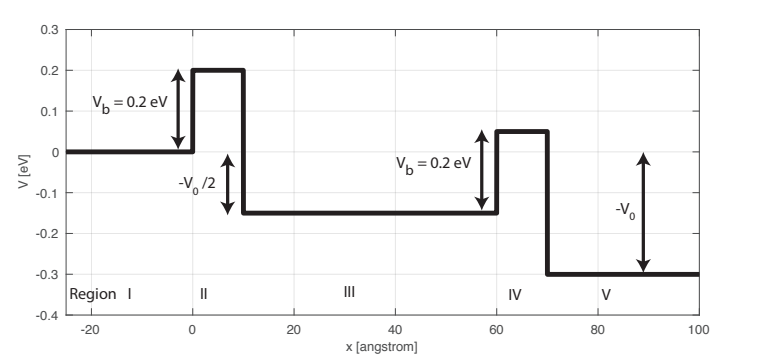
\includegraphics[width=\textwidth]{9.png}

We're given an electron with kinetic energy $0.1eV$ traveling into the potential;\\

\[
  V(x) =
  \begin{cases}
    0  & x<0 \\
    0.2eV & 0<x<10\AA\\
    -V_0/2 & 10\AA<x<60\AA\\
    -V_0/2+0.2eV & 60\AA<x<70\AA\\
    -V_0 & x>70\AA
  \end{cases}
\]
\subsection*{9a}
Substituting a plane wave into the Schrodinger equation and solving for $\psi(x)$\\

$\psi''(x)=\frac{2m}{\hbar^2}(V(x)-E)\psi(x)\Longrightarrow\psi(x)=exp(\sqrt{\frac{2m}{\hbar^2}(V(x)-E)}x)+exp(-\sqrt{\frac{2m}{\hbar^2}(V(x)-E)}x)$\\

Note this is only mathematically valid because $V(x)$ only has constant values.\\

In our 5 regions, we have 5 distinct wavefunctions with corresponding coefficients;\\

$\psi_i(x)=\alpha_ie^{k_ix}+\beta_ie^{-k_ix}$, where we have $k_i=\sqrt{\frac{2m(V_i-E)}{\hbar^2}}$\\

Note that $V_i$ is the potential in the $i$'th region.\\

\subsection*{9b}
To solve for our constants $\alpha_i$ and $\beta_i$ we use the following boundary conditions;\\

$\psi_i(x_i)=\psi_{i+1}(x_i)$, and $\frac{d\psi_i}{dx}(x_i)=\frac{d\psi_{i+1}}{dx}(x_i)$\\

Where $x_i$ is the location of the boundary between the $i$ and $i+1$'th regions\\

For all of our wave functions, $V_i>E\Rightarrow k_i\in\mathbb{R}$ and $V_i<E\Rightarrow k_i\in\mathbb{C}$, which corresponds to $\psi$ being a combination of exponential growths/decays or travelling waves, respectively. 

%We can definitively say that $V_2>E$ and thus $\psi_2(x)$ is exponential. The probability density \textit{increasing} within the barrier violates our physical intuition, and thus $\alpha_2=0$\\

In the first region, we know for a fact the electron is travelling from the left, thus our constant for $\alpha_1=1$, we can eliminate this from our list of unknowns.

In Region V, treating $\psi_5(x)=\alpha_5e^{k_Vx}+\beta_Ve^{-k_5x}$ as a sum of incident and reflected waves, it is obvious there is no barrier to reflect from, $\Rightarrow\beta_5=0$\\

%We can treat the coefficients in regions I and V as reflection and transmission constants

Now, we have reduced the number of unknown coefficients to 8, and we have 8 linear equations from our two continuity conditions from each of the four boundaries. We set up the following matrix representing our remaining coefficients in MATLAB and run the following code;\\
n=1\\
for V0=0.0:0.01:2.0\\
k1=sqrt(-0.1/3.81);\\
k2=sqrt(0.1/3.81);\\
k3=sqrt((-V0/2-0.1)/3.81);\\
k4=sqrt((0.1-V0/2)/3.81);\\
k5=sqrt((-V0-0.1)/3.81);\\
A = [\\
1,-1,-1,0,0,0,0,0;\\
k1,k2,-k2,0,0,0,0,0;\\
0,exp(10*k2),exp(-10*k2),-exp(10*k3),-exp(-10*k3),0,0,0;\\
0,k2*exp(10*k2),-k2*exp(10*k2),-k3*exp(10*k3),k3*exp(-10*k3),0,0,0;\\
0,0,0,exp(60*k3),exp(-60*k3),-exp(60*k4),-exp(-60*k4),0;\\
0,0,0,k3*exp(60*k3),-k3*exp(-60*k3),-k4*exp(60*k4),k4*exp(60*k4),0;\\
0,0,0,0,0,exp(70*k4),exp(-70*k4),-exp(70*k5);\\
0,0,0,0,0,k4*exp(70*k4),-k4*exp(-70*k4),-k5*exp(70*k5)];\\
[V,D]=eig(A)\\
a11=D(1,1)\\
B(n,1)=V0\\
B(n,2)=abs(a11)\\
B(n,3)=(1-abs(a11))\\
n=n+1\\
end\\

We now have a 3x201 matrix with all our data for the following two graphs of Reflection and Transmission as a function of bias voltage;\\

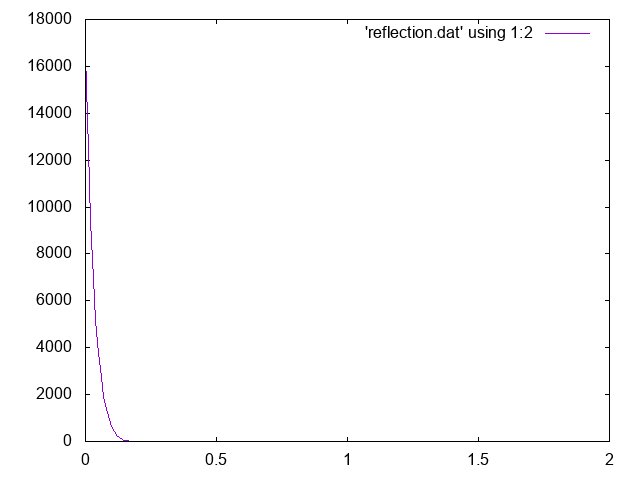
\includegraphics[width=\textwidth]{reflection.png}

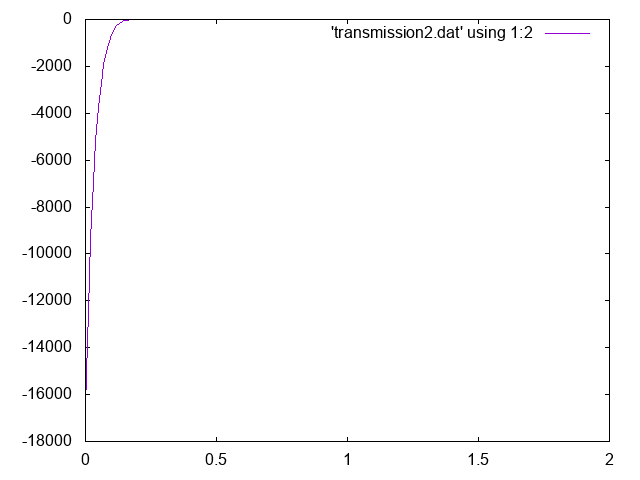
\includegraphics[width=\textwidth]{transmission.png}


\subsection*{9c}

Since there is a difference in potential between regions 1 and 5, the transmission coefficient is not simply the norm of our final coefficient\\

\subsection*{9d}

The resonances in the transmission curve occur because there is an exact multiple of wavelengths (half wavelengths to be precise) which fit between the barriers, similar to the resonant behavior of a laser entering a cavity where the cavity spacing is an integer multiple of half wavelengths.\\

\subsection*{9e}

There cannot be bound states because the potential is finite, thus there is always some finite probability for the electron to tunnel through one of the barriers.\\

\subsection*{9f}

Acknowledging the fact our above graphs do not show any resonant behavior, rather than letting this error propagate into further inaccuracies I will plead the fifth on this part of the question.

\subsection*{9g}

As the barriers increase, there is a higher and higher likelihood that the electron will reflect off each barrier, as this likelihood increases the electron can be effectively trapped and bounces off each barrier, much like how light can reflect back and forth in the cavity of a Fabry-Perot interferometer. \\

\section*{Scattering Phases and Wigner Delay}

Given the potential

\[
  V(x) =
  \begin{cases}
    0  & x<-a \\
    V_0 & -a<x\\
    \infty 0<x
  \end{cases}
\]
We can solve Schrodinger's equation to find \\

$\psi_1(x)=Ae^{ik_1x}+Be^{-ik_1x}$ where $k_1=\sqrt{\frac{2mE}{\hbar^2}}$\\

And $\psi_2(x)=Ce^{ik_2x}+De^{-ik_2x}$ where $k_2=\sqrt{\frac{2m(E-V_0)}{\hbar^2}}$\\

Note that since the potential is infinite in the rightmost region, we have $\psi(x)=0$\\

We understand that this infinite potential also causes the amplitude of our incident and reflected wave to be equal in amplitude, differing only in some scattering phase, as in $A=-Be^{i2\delta}$. We begin applying the boundary condtions;\\

$\psi_2(0)=\psi_3(0)\Rightarrow C+D=0\Rightarrow \psi_2(x)=C(e^{ik_2x}-e^{-ik_2x})=C'sin(k_2x)$\\

$\psi_1(-a)=\psi_2(-a)\Rightarrow A(e^{-ik_1a}-e^{i(2\delta+k_1a)})=-C'sink_2a$\\

$\psi_1'(-a)=\psi_2'(-a)\Rightarrow ik_1A(-e^{-ik_1a}+e^{i(2\delta+k_1a)})=-ik_2C'cosk_2a$\\

Dividing these two equations and rearranging the terms yields the following;\\

$(k_1+ik_2cot(k_2a))e^{ik_1a}=-e^{i2\delta}(k_1-ik_2cot(k_2a))e^{-ik_2a}$\\

$\Leftrightarrow B=A\frac{k_1-ik_2cotk_2a}{k_1+ik_2cotk_2a}e^{-i2k_1a}$\\

\subsection*{10b}

Taking the norm of the above equation for B, first we need to bring the imaginary unit into the numerator;\\

$ B=A\frac{k_1^2-2ik_1k_2cotk_2a-k_2^2cot^2k_2a}{k_1^2+k_2^2cot^2k_2a} $, and $ |B|=B^*B=A*A\frac{(k_1^2k_2^2cot^2k_2a)^2+4k_1^2k_2^2cot^2k_2a}{(k_1^2+k_2^2cot^2k_2a)^2} $\\

$=A^*A\frac{k_1^4+2k_1^2k_2^2cot^2k_2a+k_2^4cot^4k_2a}{(k_1^2+k_2^2cot^2k_2a)^2}=A^*A=|A|$ Thus, we have $|B|=|A|$ as we expected.\\

\subsection*{10c}
Solving for $\delta$, we achieve the following expression;\\

$\delta=(ln\frac{m1(E)}{m2(E)}-2ika)/2i$ where $m2/1(E)=k_1\pm ik_2cotk_2a$\\

For ease of computation, we set $\hbar=a=m=1$\\
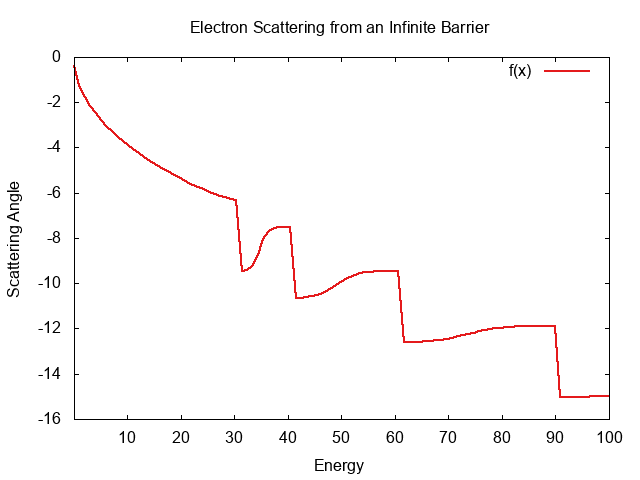
\includegraphics[width=\textwidth]{veryverylast.png}
\subsection*{10d}

We numerically derive this equation using the following definition;\\

$f'(x)=\lim_{x\rightarrow0}\frac{f(x+\Delta)-f(x)}{\Delta}$\\

Approximating this by using $\Delta=0.00001$ we get the following plot for Wigner Delay;\\
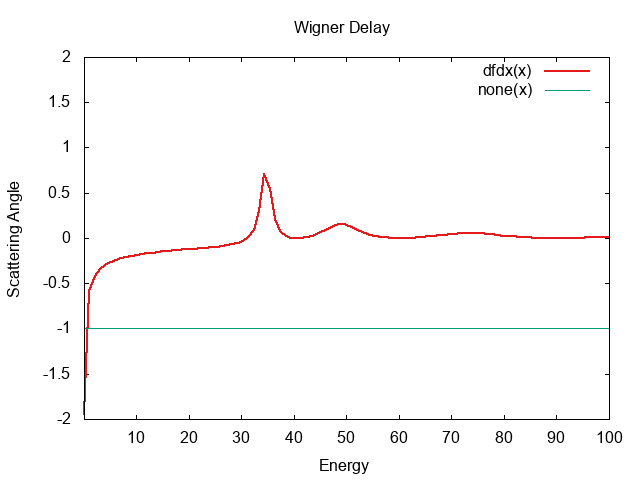
\includegraphics[width=\textwidth]{lastdfdx_tru.png}

The reason it crosses the boundary of $\frac{-a}{(\hbark/m)}$ is because of the inexact nature of our numerical derivative.\\

\end{document}

